% PREAMBLE
\documentclass{article}
% ~ ~ ~ ~ ~ ~ ~ ~ ~ ~ ~ ~ ~ ~ ~ ~ ~ ~ ~ ~ ~ ~ ~ ~ ~ ~ ~ ~ ~ ~ ~ ~ ~ ~ ~ ~ ~ ~ ~ ~ ~ ~ ~ ~ ~ ~ ~ ~

\usepackage[utf8]{inputenc}
\usepackage{amsmath}
\usepackage{amssymb} % for \mathbb
\usepackage{graphicx} % for figures
\usepackage{color}
\usepackage[usenames,dvipsnames]{xcolor}
\usepackage{hyperref} % for hyperlinks
\usepackage{float} % for figures
% ~ ~ ~ ~ ~ ~ ~ ~ ~ ~ ~ ~ ~ ~ ~ ~ ~ ~ ~ ~ ~ ~ ~ ~ ~ ~ ~ ~ ~ ~ ~ ~ ~ ~ ~ ~ ~ ~ ~ ~ ~ ~ ~ ~ ~ ~ ~ ~
% CUSTOM COLOUR
\definecolor{DGrey}{rgb}{0.1,0.1,0.1} % Dark Grey
% ~ ~ ~ ~ ~ ~ ~ ~ ~ ~ ~ ~ ~ ~ ~ ~ ~ ~ ~ ~ ~ ~ ~ ~ ~ ~ ~ ~ ~ ~ ~ ~ ~ ~ ~ ~ ~ ~ ~ ~ ~ ~ ~ ~ ~ ~ ~ ~
\title{ Introduction to Engineering Written Assignment Questions}
\date{January 2013}
\author{Greg Mayer and Daniel Connelly}
% ~ ~ ~ ~ ~ ~ ~ ~ ~ ~ ~ ~ ~ ~ ~ ~ ~ ~ ~ ~ ~ ~ ~ ~ ~ ~ ~ ~ ~ ~ ~ ~ ~ ~ ~ ~ ~ ~ ~ ~ ~ ~ ~ ~ ~ ~ ~ ~
% HEADER/FOOTER
\usepackage{fancyheadings}
\pagestyle{myheadings} % set headings to be user defined
\fancyhead{} % To create custom header, clear default layout
\renewcommand{\subsectionmark}[1]{\markright{{\color{DGrey}\thesubsection} \ {\color{DGrey}#1}}}
\fancyhead[LE,LO]{\subsectionmark} % To create custom header, clear default layout

% ~ ~ ~ ~ ~ ~ ~ ~ ~ ~ ~ ~ ~ ~ ~ ~ ~ ~ ~ ~ ~ ~ ~ ~ ~ ~ ~ ~ ~ ~ ~ ~ ~ ~ ~ ~ ~ ~ ~ ~ ~ ~ ~ ~ ~ ~ ~ ~
% ENUMERATION

\usepackage{enumitem}   % so that question numbers can be formatted 
\setenumerate[1]{label=\thesubsection.\arabic*.} % enumerate environment: add section numbers to items
% ~ ~ ~ ~ ~ ~ ~ ~ ~ ~ ~ ~ ~ ~ ~ ~ ~ ~ ~ ~ ~ ~ ~ ~ ~ ~ ~ ~ ~ ~ ~ ~ ~ ~ ~ ~ ~ ~ ~ ~ ~ ~ ~ ~ ~ ~ ~ ~
% MARGINS
\usepackage{anysize}
\marginsize{2.5cm}{2.5cm}{1cm}{1cm}
% ~ ~ ~ ~ ~ ~ ~ ~ ~ ~ ~ ~ ~ ~ ~ ~ ~ ~ ~ ~ ~ ~ ~ ~ ~ ~ ~ ~ ~ ~ ~ ~ ~ ~ ~ ~ ~ ~ ~ ~ ~ ~ ~ ~ ~ ~ ~ ~
% PAGE NUMBERING
\pagenumbering{arabic}
% ~ ~ ~ ~ ~ ~ ~ ~ ~ ~ ~ ~ ~ ~ ~ ~ ~ ~ ~ ~ ~ ~ ~ ~ ~ ~ ~ ~ ~ ~ ~ ~ ~ ~ ~ ~ ~ ~ ~ ~ ~ ~ ~ ~ ~ ~ ~ ~
% Custom Commands
\newcommand{\Emph}[1]{\textbf{#1}} % Emphasize
\newcommand{\R}{\mathbb{R}} 
\newcommand{\BM}{\begin{bmatrix}} % Begin Matrix
\newcommand{\EM}{\end{bmatrix}} % End Matrix
\newcommand{\BEN}{\begin{enumerate}[leftmargin=1.1cm]}% Begin ENumerate
\newcommand{\EEN}{\end{enumerate}} % End ENumerate
\newcommand{\MB}{\mathbf} % Math Bold

\newcommand{\px}{\frac{\partial}{\partial x}} % Partial wrt x
\newcommand{\py}{\frac{\partial}{\partial y}} % Partial wrt y

\newcommand{\pfx}{\frac{\partial f}{\partial x}} % Partial of f wrt x
\newcommand{\pfy}{\frac{\partial f}{\partial y}} % Partial of f wrt y
\newcommand{\pfxy}{\frac{\partial^2 f}{\partial y \partial x}} % Partial of f wrt y
\newcommand{\pfyx}{\frac{\partial^2 f}{\partial x \partial y}} % Partial of f wrt y

\newcommand{\ux}{\frac{\partial u}{\partial x }} % Partial of u wrt x
\newcommand{\uk}{\frac{\partial u}{\partial k }} % Partial of u wrt k
\newcommand{\ut}{\frac{\partial u}{\partial t}} % Partial of u wrt t
\newcommand{\utt}{\frac{\partial^2u}{\partial t^2}} % Partial of u wrt t
\newcommand{\us}{\frac{\partial u}{\partial s}} % Partial of u wrt t
\newcommand{\uss}{\frac{\partial^2 u}{\partial s^2}} % Partial of u wrt t
\newcommand{\kx}{\frac{\partial k}{\partial x }} % Partial of k wrt x
\newcommand{\kt}{\frac{\partial k}{\partial t }} % Partial of k wrt t

\newcommand{\pxu}{\frac{\partial x}{\partial u}} % x wrt u
\newcommand{\pxv}{\frac{\partial x}{\partial v}} % x wrt v
\newcommand{\pxw}{\frac{\partial x}{\partial w}} % x wrt v
\newcommand{\pxt}{\frac{\partial x}{\partial t}} % x wrt t
\newcommand{\pyu}{\frac{\partial y}{\partial u}} % y wrt u
\newcommand{\pyv}{\frac{\partial y}{\partial v}} % y wrt v
\newcommand{\pyw}{\frac{\partial y}{\partial w}} % y wrt v
\newcommand{\pyt}{\frac{\partial y}{\partial t}} % y wrt t
\newcommand{\pzu}{\frac{\partial z}{\partial u}} % z wrt u
\newcommand{\pzv}{\frac{\partial z}{\partial v}} % z wrt v
\newcommand{\pzw}{\frac{\partial z}{\partial w}} % z wrt v
\newcommand{\pzt}{\frac{\partial z}{\partial t}} % z wrt t


\newcommand{\VCT}{\textit{Vector Calculus} by Michael Corral} % Vector Calculus Textbook
\newcommand{\CAT}{\textit{College Algebra} by Carl Stitz and Jeff Zeager} % College Algebra Textbook
\newcommand{\From}{The following questions are related to } % Questions ....
% ~ ~ ~ ~ ~ ~ ~ ~ ~ ~ ~ ~ ~ ~ ~ ~ ~ ~ ~ ~ ~ ~ ~ ~ ~ ~ ~ ~ ~ ~ ~ ~ ~ ~ ~ ~ ~ ~ ~ ~ ~ ~ ~ ~ ~ ~ ~ ~
% ONLY USED FOR EDITING
\newcommand{\rednote}[1]{{\color{red}\textit{\textbf{#1}}}} % Shortcut for formatting notes for developers
\newcommand{\FromC}[1]{{\color{DGrey}\textit{#1}}} % Shortcut for coloring the "from" text
% ~ ~ ~ ~ ~ ~ ~ ~ ~ ~ ~ ~ ~ ~ ~ ~ ~ ~ ~ ~ ~ ~ ~ ~ ~ ~ ~ ~ ~ ~ ~ ~ ~ ~ ~ ~ ~ ~ ~ ~ ~ ~ ~ ~ ~ ~ ~ ~
% AUGMENTED MATRIX MACRO
% thanks to http://tex.stackexchange.com/questions/2233/whats-the-best-way-make-an-augmented-coefficient-matrix
\newenvironment{amatrix}[1]{%
  \left[\begin{array}{@{}*{#1}{c}|c@{}}
}{%
  \end{array}\right]
}
% ~ ~ ~ ~ ~ ~ ~ ~ ~ ~ ~ ~ ~ ~ ~ ~ ~ ~ ~ ~ ~ ~ ~ ~ ~ ~ ~ ~ ~ ~ ~ ~ ~ ~ ~ ~ ~ ~ ~ ~ ~ ~ ~ ~ ~ ~ ~ ~
% PAGE LAYOUT
\addtolength{\topmargin}{10pt}
\addtolength{\headsep}{10pt}
\addtolength{\textheight}{-20pt}


\title{Assignment 2}
\date{}

\begin{document}
\begin{center}
\textsc{\LARGE Written Assignment 1}\\[0.5cm]
\end{center}
\From sections 1.2 to 1.5 (inclusive) of \VCT.

\section*{Questions}

\begin{enumerate}
%%%%%%%%%%%%%%%%%%%%%%%%%%%%%%%%%%%%%%
%%%%%%%%%%%%%%%%%%%%%%%%%%%%%%%%%%%%%%
%%%%%%%%%%%%%%%%%%%%%%%%%%%%%%%%%%%%%%

\item 
% EASY
% GPS: MMCA1a
Find vector equations for the following lines.
\begin{enumerate}
\item Find the vector equation for the line that passes through the points (-1,2,1), and (3,-2,1).
\item Find the vector equation for the line that has parametric equations $x=2+2t, y=9t, z=5+t$.
\end{enumerate}
% -  -  -  -  -  -  -  -  -  -  -  -  -  -  -  -  -  -  -  -  -  -  -  -  -  -  -  -  -  -  
\item 
% EASY
% GPS: MMCA1a
Calculate the following angles.
\begin{enumerate}
\item Calculate the angle between the vectors $\BM -1\\ 0 \\ 1 \EM$, and $\BM 0 \\ -2 \\ 2 \EM$.
\item Calculate the angle between the vector $\mathbf{x}=\BM 1 \\ 0 \\ 2 \EM$ and the plane $2x+y-z=0$.
\end{enumerate}
% -  -  -  -  -  -  -  -  -  -  -  -  -  -  -  -  -  -  -  -  -  -  -  -  -  -  -  -  -  -  
\item 
% GPS: MMCA1ab
Find the distance between the point (1,0,0) and the line $x=1, y=t, z=1$.
% -  -  -  -  -  -  -  -  -  -  -  -  -  -  -  -  -  -  -  -  -  -  -  -  -  -  -  -  -  -  
\item 
Consider the point $(-1,C,1)$ and the plane $2x+y-z=3$, where $C$ is an unknown constant. Find all possible values of $C$ such that the distance between the given point and plane is equal to $\sqrt{6}$. 
% -  -  -  -  -  -  -  -  -  -  -  -  -  -  -  -  -  -  -  -  -  -  -  -  -  -  -  -  -  -  
\item 
%GPS: MMCA1b 
Consider the points $P, Q, R$ \\
\begin{align*}
P &=(1,0,3)\\
Q &=(2,2,3)\\
R &=(0,0,-1)
\end{align*}
\begin{enumerate}
\item Find a vector that is perpendicular to the plane that passes through these points.
\item Find the area of the triangle $\bigtriangleup PQR$.
\item Find a point $S$ so that a unique plane that passes through $P, Q$, and $S$ cannot be found. Describe why you cannot find a unique plane that passes through $P, Q$, and $S$. 
\end{enumerate}
% -  -  -  -  -  -  -  -  -  -  -  -  -  -  -  -  -  -  -  -  -  -  -  -  -  -  -  -  -  -  
\item % QUESTION 
Find two unit vectors perpendicular to vectors $\begin{bmatrix} 1 \\ 0\\4 \end{bmatrix}$ and $\mathbf{i}-2\mathbf{j}+\mathbf{k}$. 
% -  -  -  -  -  -  -  -  -  -  -  -  -  -  -  -  -  -  -  -  -  -  -  -  -  -  -  -  -  -  
\item 
Suppose vectors $\mathbf{a}$, $\mathbf{b}$, and $\mathbf{c}$ are in $\mathbb{R}^3$, and \textbf{a}$\ne 0$. If \textbf{a}$\cdot\mathbf{b}=\mathbf{a}\cdot\mathbf{c}$, does it follow that $\mathbf{b}=\mathbf{c}$? Briefly explain your answer. 
% -  -  -  -  -  -  -  -  -  -  -  -  -  -  -  -  -  -  -  -  -  -  -  -  -  -  -  -  -  -  
\item % QUESTION 
Find the equation of the plane that
\begin{enumerate}
\item passes through the points (-1,2,1), (3,-2,1), and (-1,1,-1).
\item passes through the point (-1,2,1) and contains the line $x=y=z$.
\end{enumerate}
% -  -  -  -  -  -  -  -  -  -  -  -  -  -  -  -  -  -  -  -  -  -  -  -  -  -  -  -  -  -  
\item % QUESTION 
Suppose we have two planes $2x+y-z=3$ and $x+3y+z=0$. Find the line of intersection between these two planes, and find the equation of the plane that passes through the line of intersection and through the point $(0,0,0)$.
% -  -  -  -  -  -  -  -  -  -  -  -  -  -  -  -  -  -  -  -  -  -  -  -  -  -  -  -  -  -  
\item % QUESTION
Suppose that $L_1$ is a line in $\R^3$.
\begin{enumerate}
\item Is it possible to find another line, $L_2$, that is parallel $L_1$, and intersects $L_1$ at only one point? Show that it is  possible, or show that it is not possible with a counterexample.
\item Suppose that there is a line $L_3$ that is is parallel to $L_1$, and that a plane $P$ includes both $L_1$ and $L_3$. Is it always true that there exists a plane that is perpendicular to $P$? 
\end{enumerate}
% -  -  -  -  -  -  -  -  -  -  -  -  -  -  -  -  -  -  -  -  -  -  -  -  -  -  -  -  -  -  
\item % QUESTION 
Consider the following vectors in $\R^2$:
\begin{align*}
\mathbf{a} = \begin{bmatrix} 1/\sqrt{2} \\ -1/\sqrt{2} \end{bmatrix}, \quad
\mathbf{b} = \begin{bmatrix} 1/\sqrt{2} \\ 1/\sqrt{2} \end{bmatrix}, \quad
\mathbf{r} =  \begin{bmatrix} 3 \\ 1 \end{bmatrix}.
\end{align*}
\begin{enumerate}
\item Verify that $\mathbf{a}$ and $\mathbf{b}$ are perpendicular unit vectors. 
\item Use your results from part (a) to find constants $C_1$ and $C_2$ so that $\mathbf{r}=C_1\mathbf{a}+C_2\mathbf{b}$.
\end{enumerate}
% -  -  -  -  -  -  -  -  -  -  -  -  -  -  -  -  -  -  -  -  -  -  -  -  -  -  -  -  -  -  
\item % QUESTION 
Suppose that $\mathbf{a}$, $\mathbf{b}$ and $\mathbf{c}$ are nonzero vectors in $\R^3$. Prove the following statements.
\begin{enumerate}
\item If $||\mathbf{a} + \mathbf{b}||^2 = ||\mathbf{a}||^2 + ||\mathbf{b}||^2$, then vectors $\mathbf{a}$ and $\mathbf{b}$ are perpendicular. 
\item If $\mathbf{a}\times\mathbf{b} = \mathbf{a}\times\mathbf{c}$ and $\mathbf{a}\cdot\mathbf{b} = \mathbf{a}\cdot\mathbf{c}$, then $\mathbf{b} =\mathbf{c}$.
\end{enumerate}
% -  -  -  -  -  -  -  -  -  -  -  -  -  -  -  -  -  -  -  -  -  -  -  -  -  -  -  -  -  -  
\item 
Suppose that $\mathbf{a}$, $\mathbf{b}$ and $\mathbf{c}$ are nonzero vectors in $\R^3$. Identify which of the following statements are meaningless and which statements are not meaningless. Explain your reasoning.
\begin{enumerate}
\item  $\mathbf{a}\cdot (\mathbf{b} \times \mathbf{c})$ 
\item  $\mathbf{a}\cdot (\mathbf{b} \cdot \mathbf{c})$ 
\item  $\mathbf{a}\times (\mathbf{b} \cdot \mathbf{c})$ 
\item  $\mathbf{a}\times (\mathbf{b} \times \mathbf{c})$ 
\end{enumerate}
% -  -  -  -  -  -  -  -  -  -  -  -  -  -  -  -  -  -  -  -  -  -  -  -  -  -  -  -  -  -  
\item \textbf{Application to Mechanics, Part I} \\
Torque plays a fundamental role in many branches of engineering. It is vector that describes rotation rotation about a point or axis due to an applied force. If you haven't yet encountered torque, its mathematical definition is straightforward:
\begin{quote}
The torque, $\boldsymbol\tau$, about a pivot point $P$, that is produced by a force \textbf{F} applied at a point $Q$, is defined as $\boldsymbol\tau = \mathbf{r} \times \mathbf{F}$, where $\mathbf{r}=\overrightarrow{PQ}$.
\end{quote}
Torque is a vector that is produced by an applied force. For example, suppose that a force $\MB{F}=\frac{1}{2}\MB{i} + 0\MB{j} + 0\MB{k}$ is applied at the point $(1,C,0)$, about the pivot point (1,0,0), where $C\in\R$ is a constant. The resulting torque is simply 
\begin{align*}
\boldsymbol\tau =   
\begin{vmatrix}
   \MB{i} &  \MB{j} &  \MB{k} \\
   1-1 &  C-0 &  0 \\
   0.5 & 0 &  0 \\
  \end{vmatrix}=-\frac{C}{2}\MB{k}
\end{align*} 
A plot of the applied force and produced torque vectors is shown below.
\begin{figure}[!htbp]
  \begin{center}
    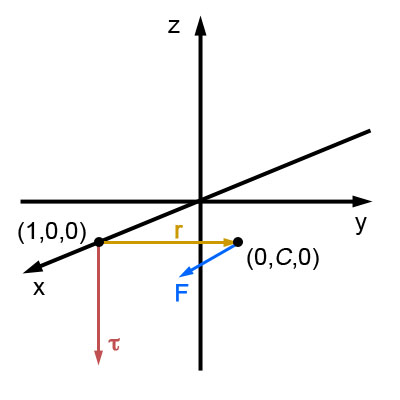
\includegraphics[width=0.5\textwidth]{WA01TorqueExample.jpg}
  \end{center}
\end{figure}

Note that the magnitude of the torque vector is $||\boldsymbol\tau|| = C/2$, and that if we increase the value of $C$, two things happen: the applied force moves further away from the pivot point, and the magnitude of the produced torque increases. \\\\
% Consider that:
%\begin{itemize}
%\item intuitively, it is easier to rotate a screwdriver with a \textbf{large} handle than it is to rotate a screwdriver a small handle. If the 
%\item It is easier to spin a large wheel by pushing on its edge, rather than pushing on some point in the middle of the wheel. Moreover, we 
%\end{itemize}
\textbf{Units}\\
When \textbf{F} has units of Newtons (N), and $\MB{r}$ has units of meters (m), torque has units of $\text{N}\cdot\text{m}$.\\\\
\textbf{Questions}\\
Suppose that a bicycle has pedal arms that are 0.14 m long, and that a constant downward force of $100 \text{ N}$ is applied by a cyclist on one pedal.  Let $\theta \in [0,360^{\circ})$ be the angle between the vertical and the pedal arm, as shown in the figure below. 
\begin{figure}[!htbp]
  \begin{center}
    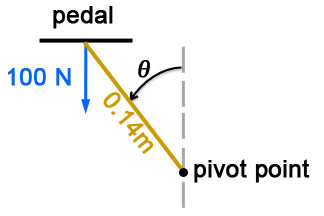
\includegraphics[width=0.4\textwidth]{WA01Bicycle.jpg}
      \caption{\small{The pedal arm (orange) rotates about the pivot point. The angle it makes with the vertical direction is $\theta$, measured counter-clockwise. A constant downward force of 100 N is applied to the pedal, which is attached to the other end of the pedal arm.}}
  \end{center}
\end{figure}
\BEN
  \item Determine the magnitude of the torque about the pivot point when $\theta$ is $30^{\circ}$ and when $\theta$ is $90^{\circ}$. Your answers should include the units of measurement. 
  \item Determine the magnitude of the torque about the pivot point for any $\theta$. Your answer should be a function of $\theta$.  
  \item What value(s) of $\theta$ minimize the produced torque? Briefly explain why. You should not need to compute any derivatives to answer this question. 
\EEN
Naturally, the torque vector can also be a function of time. In our bicycle example, the torque that is produced by the cyclist could change continuously as the pedal rotates about the pivot point. We will revisit the concept of torque as a vector function in a later assignment, after we have defined vector functions and their derivatives. 

%% -  -  -  -  -  -  -  -  -  -  -  -  -  -  -  -  -  -  -  -  -  -  -  -  -  -  -  -  -  -  

\end{enumerate}

%%%%%%%%%%%%%%%%%%%%%%%%%%%%%%%%%%%%%%
%%%%%%%%%%%%%%%%%%%%%%%%%%%%%%%%%%%%%%
%%%%%%%%%%%%%%%%%%%%%%%%%%%%%%%%%%%%%%


% SOLUTIONS
\newpage
\section*{Solutions}

\begin{enumerate}
% ~~~~~~~~~~~~~~~~~~~~~~~~~~~~~~~~~~~~~~~~~~~~~~~~~~~~~~~~~
\item
\begin{enumerate}
\item 

A vector parallel to the required line is given by $\BM 3\\ -2\\1\EM - \BM -1 \\2 \\ 1\EM  = \BM 4 \\-4 \\0 \EM$. If we like, for simplicity, we can normalize this vector by dividing each component by 4 to obtain the vector $[1,-1,0]^T$. Since a point on the desired line is (-1,2,1), a vector equation is given by 
\begin{align*}
\mathbf{r}=\BM-1 \\2 \\1\EM+t\BM1 \\ -1 \\0 \EM.
\end{align*}
The solution to this question is not unique. Any vector parallel to the vector $\BM 4 \\ -4 \\ 0 \EM$ could be used. 

% -  -  -  -  -  -  -  -  -  -  -  -  -  -  -  -  -  -  -  -  -  -  -  -  -  -  -  -  -  -  
\item 
A vector equation is 
\begin{align*}
\mathbf{r} &= (2+2t)\mathbf{i} + (9t)\mathbf{j} + (5+t)\mathbf{k} \\
&= (2\mathbf{i} + 5\mathbf{k}) + t(2\mathbf{i} + 9\mathbf{k} + \mathbf{k}) \\
&= \BM 2 \\ 0 \\ 5 \EM + t \BM 2 \\ 9 \\1 \EM
\end{align*}
\end{enumerate}
% ~~~~~~~~~~~~~~~~~~~~~~~~~~~~~~~~~~~~~~~~~~~~~~~~~~~~~~~~~
\item
% -  -  -  -  -  -  -  -  -  -  -  -  -  -  -  -  -  -  -  -  -  -  -  -  -  -  -  -  -  -  
\begin{enumerate}
\item 
Let $\mathbf{A} = \BM-1 \\ 0 \\ 1\EM$ and $\mathbf{B} = \BM 0 \\ -2 \\ 2 \EM$. Then
\begin{align*}
  \mathbf{A} \cdot \mathbf{B} &= \big((-1)(0)\big) + \big((0)(-2)\big) + \big((1)(2)\big)\\
  &= 0 + 0 + 2 \\
  &= 2
\end{align*}
Also,
\begin{align*}
  || \mathbf{A} || &= \sqrt{(-1)^2 + 0 + (1)^2} = \sqrt{2} \\
  || \mathbf{B} || &= \sqrt{0^2 + (-2)^2 + 2^2} = \sqrt{8}
\end{align*}
Therefore, if $\theta$ is the angle between the two vectors, 
\begin{align*}
  \cos\theta &= \frac{ \mathbf{A}\cdot \mathbf{B}}{|| \mathbf{A}|| \ || \mathbf{B}||} = \frac{2}{4} = \frac{1}{2}
\end{align*}
Therefore, $\theta = \pi/3$. 

% -  -  -  -  -  -  -  -  -  -  -  -  -  -  -  -  -  -  -  -  -  -  -  -  -  -  -  -  -  -  
\item 
Let the vector perpendicular to the plane be $\mathbf{y}= \BM 2 \\ 1 \\ -1 \EM$. The angle, $\theta$, between the given vector and $\mathbf{y}$ is found by solving
\begin{align*}
  \cos\theta &= \frac{ \mathbf{x}\cdot \mathbf{y}}{|| \mathbf{x}|| \ || \mathbf{y}||} \\
  &= \frac{ \BM 1 \\0 \\ 2 \EM \cdot \BM 2 \\1 \\-1 \EM} {\sqrt{5}\sqrt{6}}\\
    &= \frac{ 0 } {\sqrt{5}\sqrt{6}}\\
    &=0.
\end{align*}
The angle, $\theta$, is $\pi/2$. But $\theta$ is the angle between $\mathbf{x}$ and $\mathbf{y}$ and we need the angle between $\mathbf{x}$ and the plane, which is $\pi/2 - \theta = 0$. Therefore, the desired angle is 0 (the given vector is parallel to the plane). 
\end{enumerate}

% ~~~~~~~~~~~~~~~~~~~~~~~~~~~~~~~~~~~~~~~~~~~~~~~~~~~~~~~~~
\item
Let the normal vector of the first plane be $\mathbf{n}_1$, and the normal vector of the second plane be $\mathbf{n}_2$. Then  
\begin{align*}
\mathbf{n}_1 \times \mathbf{n}_2 
&= (0-(-8))\mathbf{i} - (1-4)\mathbf{j}+(-2-0)\mathbf{k} \\
&=\BM 8 \\ 3 \\ -2 \EM
\end{align*}
This vector is perpendicular to the two given vectors. Its length is
\begin{align*}
\big|\big| [8,3,-2]^T \big|\big| 
&= \sqrt{ 8^2+3^2+(-2)^2} \\
&= \sqrt{77}
\end{align*}
Therefore, two unit vectors are
\begin{align*}
\BM 8/\sqrt{77} \\ 3/\sqrt{77}\\ -2/\sqrt{77}\EM , \text{ and } \BM -8/\sqrt{77} \\ -3/\sqrt{77} \\ 2/\sqrt{77} \EM
\end{align*}
% ~~~~~~~~~~~~~~~~~~~~~~~~~~~~~~~~~~~~~~~~~~~~~~~~~~~~~~~~~
\item
The formula we can apply is:
\begin{align*}
  D = \frac{||\mathbf{v} \times \mathbf{w}||}{|| \mathbf{v}||}
\end{align*}
where $\mathbf{v}$ is a vector parallel to the given line, and is
\begin{align*}
  \mathbf{v} &= \BM 0 \\ 1 \\ 0 \EM.
\end{align*}
The vector $\mathbf{w}$ is
\begin{align*}
  \mathbf{w} &= \BM 1 \\ 0 \\ 0 \EM  - \BM 1 \\ 0 \\ 1 \EM = \BM 0\\0\\-1 \EM
\end{align*}
Then,
\begin{align*}
  D & = \frac{||\mathbf{v} \times \mathbf{w}||}{|| \mathbf{v}||} \\
  &= \frac{||[ -1,0,0 ] ^T||}{|| [0,1,0]^T||}\\
  &= \frac{1}{1}\\
  &= 1
\end{align*}
% ~~~~~~~~~~~~~~~~~~~~~~~~~~~~~~~~~~~~~~~~~~~~~~~~~~~~~~~~~
\item 
The formula we can apply is:
\begin{align*}
  D = \frac{| ax_0 + by_0 +cz_0 +d|}{\sqrt{a^2+b^2+c^2}}
\end{align*}
where $a, b, c$ are the components of the normal vector to the plane, so that
\begin{align*}
  \BM a \\ b \\ c \EM = \BM 2 \\ 1 \\ -1 \EM
\end{align*}
The point $(x_0,y_0,z_0) = (-1 , C, 1)$, $d = -3$, and $D = \sqrt{6}$. Thus,
\begin{align*}
  D = \sqrt{6} &= \frac{| 2(-1) + C(1) + (1)(-1) -3|}{\sqrt{6}}\\
  &= \frac{| C - 6|}{\sqrt{6}}\\
  1 &= | C - 6| \\
\end{align*}
Therefore, $C = 5, 7$.
% ~~~~~~~~~~~~~~~~~~~~~~~~~~~~~~~~~~~~~~~~~~~~~~~~~~~~~~~~~
\item  % SOLUTION
\begin{enumerate}
\item
We can start by finding the plane that contains the three points. The vectors $\overrightarrow{PQ}$ and $\overrightarrow{PR}$ are 

\begin{align*}
\overrightarrow{PQ} &= \BM 2 \\ 2 \\ 3 \EM - \BM 1 \\ 0 \\ 3 \EM  = \BM 1 \\ 2 \\ 0 \EM \\
\overrightarrow{PR} &= \BM 0 \\ 0 \\ -1 \EM - \BM 1 \\ 0 \\ 3 \EM  =  \BM -1 \\ 0 \\ -4 \EM
\end{align*}

A vector perpendicular to the plane that contains the three points is found by calculating the cross product between these two vectors:
\begin{align*}
\overrightarrow{PQ} \times \overrightarrow{PR} 
&= (-8-(0))\mathbf{i} - (-4-0)\mathbf{j}+(0-(-2))\mathbf{k} \\
&= \BM -8 \\ 4 \\ 2 \EM
\end{align*}
Any vector parallel to this vector is perpendicular to the plane that contains the given points. 
% -  -  -  -  -  -  -  -  -  -  -  -  -  -  -  -  -  -  -  -  -  -  -  -  -  -  -  -  -  -  
\item
To find the area, $A$, of  triangle $\bigtriangleup PQR$, we can use a cross product.
\begin{align*}
A &= \frac{1}{2} \big|\big| \overrightarrow{PQ} \times \overrightarrow{PR} \big|\big| \\
&= \frac{1}{2} \big|\big| [-8,4,2]^T \big|\big| \\
&= \frac{1}{2} \sqrt{ (-8)^2+4^2+2^2} \\
&= \frac{1}{2} \sqrt{ 84} \ \\
&= \sqrt{21} \\
\end{align*}
% -  -  -  -  -  -  -  -  -  -  -  -  -  -  -  -  -  -  -  -  -  -  -  -  -  -  -  -  -  -  
\item
If the point $S$ is such that $\overrightarrow{PQ}$ is parallel to $\overrightarrow{QS}$, then there will be an infinite number of planes that pass through these three points. Such a point, $S$, can be determined by multiplying $\overrightarrow{PQ}$ by a constant. Choosing 2 as a constant, then 
\begin{align*}
\overrightarrow{QS} &= \BM 2 \\ 4 \\ 0 \EM\\
\end{align*}
We determine the components of $S$ as
\begin{align*}
S &= \BM 2-2 \\ 4-2 \\ 0-3 \EM = \BM 0 \\ 2 \\ -3 \EM\\
\end{align*}
\end{enumerate}

% ~~~~~~~~~~~~~~~~~~~~~~~~~~~~~~~~~~~~~~~~~~~~~~~~~~~~~~~~~


\item
It is not necessarily true that $\mathbf{b}=\mathbf{c}$. Simple rearrangement yields
\begin{align*}
\mathbf{a}\cdot\mathbf{b}&=\mathbf{a}\cdot\mathbf{c} \\
0 &=\mathbf{a}\cdot\mathbf{b} - \mathbf{a}\cdot\mathbf{c} \\
0 &=\mathbf{a}\cdot (\mathbf{b} - \mathbf{c})
\end{align*}
Therefore, \textbf{a} is perpendicular to the vector $\mathbf{b} - \mathbf{c}$, which can be true when $\mathbf{b} \ne \mathbf{c}$.  A counterexample would be the vectors
\begin{align*}
\mathbf{a} = \BM 1 \\ 1 \\ 0 \EM ,  \quad \mathbf{b} = \BM 1 \\ -1 \\ 0 \EM , \quad  \mathbf{c} = \BM 0 \\ 0 \\ 0 \EM .
\end{align*}
Clearly, \textbf{a}$\cdot\mathbf{b}=\mathbf{a}\cdot\mathbf{c}$, even though $\mathbf{b} \ne \mathbf{c}$.  
% ~~~~~~~~~~~~~~~~~~~~~~~~~~~~~~~~~~~~~~~~~~~~~~~~~~~~~~~~~

\item
\begin{enumerate}
\item
Let the points $P, Q, R$ be \\
\begin{align*}
P &=(-1,2,1)\\
Q &=(3,-2,1)\\
R &=(-1,1,-1)
\end{align*}
Vectors  $\overrightarrow{PQ}$ and $\overrightarrow{PR}$ are
\begin{align*}
\overrightarrow{PQ} &= \BM 3 \\ -2 \\ 1 \EM -(-1,2,1) = (4,-4,0)\\
\overrightarrow{PR} &= \BM -1 \\ 1 \\ -1 \EM - \BM -1 \\ 2 \\ 1 \EM = \BM 0 \\ -1 \\ -2\EM
\end{align*}
A vector orthogonal to the plane that contains the three points is found by calculating the cross product between these two vectors:
\begin{align*}
\overrightarrow{PQ} \times \overrightarrow{PR} 
&= (8-0)\mathbf{i} - (-8-0)\mathbf{j}+(-4-0)\mathbf{k} \\
&=(8,8,-4)
\end{align*}
The equation of the desired plane, using the point-normal form, is
\begin{align*}
0&=8(x+1)+8(y-2)+(-4)(z-1)\\
4&=8x + 8y -4z
\end{align*}

\item
The points $(0,0,0)$ and $(1,1,1)$ are on the given line. Therefore, the vector $\BM 1 \\ 1 \\1 \EM$ is parallel to the desired plane. Another vector parallel to the desired plane is 
\begin{align*}
  \BM -1 \\ 2 \\ 1 \EM - \BM 0 \\ 0 \\0 \EM = \BM -1\\2\\1\EM.
\end{align*}
Therefore, a vector perpendicular to the desired plane is 
\begin{align*}
\BM 1\\1\\1\EM  \times \BM-1\\2\\1\EM 
&= (1-2)\mathbf{i} - (1+1)\mathbf{j}+(2+1)\mathbf{k} = \BM -1 \\ -2 \\ 3 \EM .
\end{align*}
The equation of the desired plane, using the point-normal form, is
\begin{align*}
0&=-1(x+1)-2(y-2)+3(z-1)\\
0 &=-x - 2y +3z .
\end{align*}


\end{enumerate}
% ~~~~~~~~~~~~~~~~~~~~~~~~~~~~~~~~~~~~~~~~~~~~~~~~~~~~~~~~~
% EQUATION OF PLANE FROM INTERSECTION BETWEEN TWO LINES
\item

Let the normal vector of the first plane be $\mathbf{n}_1$, and the normal vector of the second plane be $\mathbf{n}_2$. Then  
\begin{align*}
\mathbf{n}_1 =\BM 2 \\ 1 \\ -1 \EM, \ 
\mathbf{n}_2=\BM 1\\ 3 \\ 1 \EM
\end{align*}
The line that intersects these two planes is a line that is in both of the planes, and therefore must be perpendicular to both $\mathbf{n}_1$ and $\mathbf{n}_2$. Therefore, the line we need is parallel to the vector, $\mathbf{a}$, given by the cross product
\begin{align*}
\mathbf{a} &= \mathbf{n}_1 \times \mathbf{n}_2 = (4,-3,5).
\end{align*}
This vector is parallel to the desired plane. To find a second vector in the desired plane, we can find a line from the given point to any point in the line of intersection of the two given planes. Letting $y=0$, we obtain the equations
\begin{align*}
2x-z&=3\\
x+z&=0
\end{align*}
which has the solution $x=1, z=-1$. Therefore, the point $(1,0,-1)$ is in the intersection of the two planes, and a vector in the plane is
\begin{align*}
\BM 1 \\ 0 \\ -1 \EM- \BM 0 \\ 0 \\ 0 \EM = \BM 1 \\ 0 \\ -1 \EM.
\end{align*}
A normal vector to the desired plane is 
\begin{align*}
[1,0,-1]^T \times [4,-3,5]^T 
&= (0-3)\mathbf{i} - (5+4)\mathbf{j}+(-3-0)\mathbf{k} \\
&=-3\mathbf{i} -9 \mathbf{j} -3\mathbf{k} 
\end{align*}
The equation of the desired plane, using the point-normal form, is
\begin{align*}
0&=(-3)(x-0)+(-9)(y-0)+(-3)(z-0)\\
&=-3x-9y-3z
\end{align*}

% ~~~~~~~~~~~~~~~~~~~~~~~~~~~~~~~~~~~~~~~~~~~~~~~~~~~~~~~~~
% ORTHOGONAL VECTORS
\item
\begin{enumerate}
% ~ ~ ~ ~ ~ ~ ~ ~ ~ ~ ~ ~ ~ ~ ~ ~ ~ ~ ~ ~ ~ ~ ~ ~ ~ ~ ~ ~ ~ ~ ~ ~ ~ ~ ~ ~ ~ ~ ~ ~ 
% PART A
\item We will show that the two lines must be equal to each other, and therefore share an infinite number of points. Let $P$ be the common point, and $\mathbf{r}$ be the vector pointing from the origin to the point $P$. Let 
\begin{align*}
  L_1 &= \mathbf{r} + t\mathbf{u} \\
  L_2 &= \mathbf{r} + t\mathbf{v} \\  
\end{align*}
where $t \in \R$, and \textbf{u} and \textbf{v} are vectors parallel to the lines $L_1$ and $L_2$ respectively. Let their components be 
\begin{align*}
\mathbf{u} = \begin{bmatrix} u_1 \\ u_2 \\ u_3 \end{bmatrix},  \quad
\mathbf{v} = \begin{bmatrix} v_1 \\ v_2 \\ v_3 \end{bmatrix} .
\end{align*}
When the lines intersect, their components are equal, which gives us the three equations 
\begin{align*}
r_1 +t u_1 &= r_1 + tv_1 \\
r_2 +t u_2 &= r_2 + tv_2 \\
r_3 +t u_3 &= r_3 + tv_3 
\end{align*}
Or simply
\begin{align*}
t u_1 &= tv_1 \\
t u_2 &= tv_2 \\
t u_3 &= tv_3 
\end{align*}
Because $L_1$ and $L_2$ are parallel, vectors \textbf{u} and \textbf{v} must also be parallel. Therefore $\mathbf{u}=k\mathbf{v}$ where $k$ is a constant, so 
\begin{align*}
t u_1 &= tku_1 \\
t u_2 &= tku_2 \\
t u_3 &= tku_3 
\end{align*}
These equations are only satisfied if $k=1$. Therefore, the two lines must be equal to each other, implying that there an infinite number of points that the two lines share. 
% ~ ~ ~ ~ ~ ~ ~ ~ ~ ~ ~ ~ ~ ~ ~ ~ ~ ~ ~ ~ ~ ~ ~ ~ ~ ~ ~ ~ ~ ~ ~ ~ ~ ~ ~ ~ ~ ~ ~ ~ 
% PART B
\item Yes. Any plane in $\R^3$ can be expressed in point-normal form 
\begin{align*}
a(x-x_0) - b(y-y_0)+c(z-z_0) = 0
\end{align*}
where the vector $\begin{bmatrix} a \\ b \\ c \end{bmatrix}$ is a vector normal to the plane. 
\end{enumerate}

% ~~~~~~~~~~~~~~~~~~~~~~~~~~~~~~~~~~~~~~~~~~~~~~~~~~~~~~~~~
% ORTHOGONAL VECTORS
\item
\begin{enumerate}
% ~ ~ ~ ~ ~ ~ ~ ~ ~ ~ ~ ~ ~ ~ ~ ~ ~ ~ ~ ~ ~ ~ ~ ~ ~ ~ ~ ~ ~ ~ ~ ~ ~ ~ ~ ~ ~ ~ ~ ~ 
% PART A
\item Vectors $\mathbf{a}$ and $\mathbf{b}$ are perpendicular because their dot product is zero:
\begin{align*}
\mathbf{a} \cdot \mathbf{b} = \frac{1}{2} -  \frac{1}{2} =0.
\end{align*}
Vectors $\mathbf{a}$ and $\mathbf{b}$ are both unit vectors, because they have length 1:
\begin{align*}
|| \mathbf{a} || &=  \sqrt{ \Bigg( \frac{1}{\sqrt{2}}\Bigg)^2 +  \Bigg(\frac{-1}{\sqrt{2}}\Bigg)^2} = 1\\
|| \mathbf{b} || &=  \sqrt{ \Bigg( \frac{1}{\sqrt{2}}\Bigg)^2 +  \Bigg(\frac{1}{\sqrt{2}}\Bigg)^2} = 1
\end{align*}
% ~ ~ ~ ~ ~ ~ ~ ~ ~ ~ ~ ~ ~ ~ ~ ~ ~ ~ ~ ~ ~ ~ ~ ~ ~ ~ ~ ~ ~ ~ ~ ~ ~ ~ ~ ~ ~ ~ ~ ~ 
% PART B
\item Using results from part (a), we can find $C_1$ as follows:
\begin{align*}
\mathbf{r} &= C_1 \mathbf{a} + C_2  \mathbf{b} \\
\mathbf{a}\cdot\mathbf{r} &=  \mathbf{a}\cdot \Big(C_1 \mathbf{a} + C_2 \mathbf{b} \Big)\\
\mathbf{a}\cdot\mathbf{r} &= C_1 \mathbf{a}\cdot \mathbf{a} + C_2\mathbf{a}\cdot   \mathbf{b} \\
\frac{2}{\sqrt{2}} &= C_1 (1) + C_2(0) \\
C_1 &= \frac{2}{\sqrt{2}} \\
\end{align*}
A similar calculation yields $C_2$
\begin{align*}
\mathbf{r} &= C_1 \mathbf{a} + C_2  \mathbf{b} \\
\mathbf{b}\cdot\mathbf{r} &=  \mathbf{b}\cdot \Big(C_1 \mathbf{a} + C_2 \mathbf{b} \Big)\\
\mathbf{b}\cdot\mathbf{r} &= C_1 \mathbf{b}\cdot \mathbf{a} + C_2\mathbf{b}\cdot   \mathbf{b} \\
\frac{4}{\sqrt{2}} &= C_1 (0) + C_2(1) \\
C_2 &= \frac{4}{\sqrt{2}} = 2\sqrt{2} \\
\end{align*}
\end{enumerate}
% ~~~~~~~~~~~~~~~~~~~~~~~~~~~~~~~~~~~~~~~~~~~~~~~~~~~~~~~~~
% TRUE/FALSE
\item
% ~ ~ ~ ~ ~ ~ ~ ~ ~ ~ ~ ~ ~ ~ ~ ~ ~ ~ ~ ~ ~ ~ ~ ~ ~ ~ ~ ~ ~ ~ ~ ~ ~ ~ ~ ~ ~ ~ ~ ~ 
% PART A
\begin{enumerate}
\item Expanding the left-hand side yields
\begin{align*}
||\mathbf{a} + \mathbf{b}||^2 &= \big(\mathbf{a} + \mathbf{b}\big)\cdot\big(\mathbf{a} + \mathbf{b}\big) \\
&= \mathbf{a}\cdot\mathbf{a} + \mathbf{b}\cdot\mathbf{b} + 2\mathbf{a}\cdot\mathbf{b}\\
&= ||\mathbf{a}||^2 + ||\mathbf{b}||^2 + 2\mathbf{a}\cdot\mathbf{b}
\end{align*}
This is equal to $ ||\mathbf{a}||^2 + ||\mathbf{b}||^2$ iff $\mathbf{a}\cdot\mathbf{b}=0$, which implies that $\mathbf{a}$ must be perpendicular to $\mathbf{b}$.
% ~ ~ ~ ~ ~ ~ ~ ~ ~ ~ ~ ~ ~ ~ ~ ~ ~ ~ ~ ~ ~ ~ ~ ~ ~ ~ ~ ~ ~ ~ ~ ~ ~ ~ ~ ~ ~ ~ ~ ~ 
\item First consider the dot product:
\begin{align*}
\mathbf{a}\cdot\mathbf{b} &= \mathbf{a}\cdot\mathbf{c} \\
0 &= \mathbf{a}\cdot\mathbf{b} - \mathbf{a}\cdot\mathbf{c} \\
0 &= \mathbf{a}\cdot\big(\mathbf{b} - \mathbf{c}\big) \\
\end{align*}
Therefore, $\mathbf{a}$ is perpendicular to the vector $\mathbf{b} - \mathbf{c}$. Manipulation of the cross product yields
\begin{align*}
\mathbf{a}\times\mathbf{b} &= \mathbf{a}\times\mathbf{c} \\
0 &= \mathbf{a}\times\mathbf{b} - \mathbf{a}\times\mathbf{c} \\
0 &= \mathbf{a}\times\big(\mathbf{b} - \mathbf{c}\big) \\
\end{align*}
Therefore, $\mathbf{a}$ is also parallel to the vector $\mathbf{b} - \mathbf{c}$. Therefore, $\mathbf{b} - \mathbf{c} = \mathbf{0}$, or $\mathbf{b} = \mathbf{c}$.
%\item The statement is false: $\BM 1 \\ 2 \\ 3 \EM = \BM 1 ,2 ,3\EM^T$.
% ~ ~ ~ ~ ~ ~ ~ ~ ~ ~ ~ ~ ~ ~ ~ ~ ~ ~ ~ ~ ~ ~ ~ ~ ~ ~ ~ ~ ~ ~ ~ ~ ~ ~ ~ ~ ~ ~ ~ ~ 
\end{enumerate}
% ~~~~~~~~~~~~~~~~~~~~~~~~~~~~~~~~~~~~~~~~~~~~~~~~~~~~~~~~~
% MEANINGLESS STATEMENTS
\item
\begin{enumerate}
\item This statement is not meaningless. This is a dot product of two vectors.
\item This statement is meaningless. We cannot take the dot product of a vector with a scalar. 
\item This statement is meaningless. We cannot take the cross product of a vector with a scalar. 
\item This statement is not meaningless. This is a cross product of two vectors.
\end{enumerate}
% ~~~~~~~~~~~~~~~~~~~~~~~~~~~~~~~~~~~~~~~~~~~~~~~~~~~~~~~~~
% TORQUE
\item
For this problem we will use the coordinate system in the diagram below. 
\begin{figure}[!htbp]
  \begin{center}
    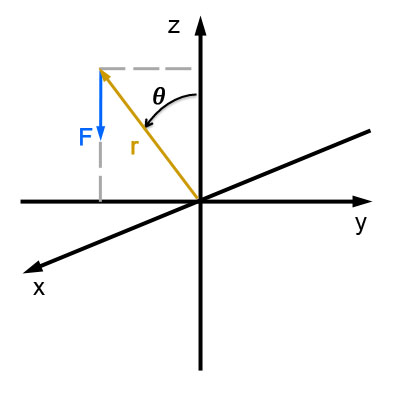
\includegraphics[width=0.4\textwidth]{WA01TorqueSol.jpg}
  \end{center}
\end{figure}
\BEN
\item Using the above coordinate system, we are given that $||\MB{r}|| = 0.14$ and $\MB{F} = -100\MB{k}$. Also, 
\begin{align*}
  \MB{r} &=- \sin(30^{\circ})||\MB{r}||\MB{j} + \cos(30^{\circ} )||\MB{r}||\MB{k}\\
  &= -0.07\MB{j} + 0.07\sqrt{3}\MB{k}\\
  &= 0.07\big(-\MB{j} + \sqrt{3}\MB{k}\big)
\end{align*}
To compute the torque when $\theta = 30^{\circ}$, we use the cross product:
\begin{align*}
0.07
\begin{vmatrix}
   \MB{i} & \MB{j} &  \MB{k} \\
   0 & -1 &  \sqrt{3} \\
   0 & 0 & -100  \\
  \end{vmatrix}=7\MB{i}
\end{align*} 
Thus, the magnitude of the torque $\boldsymbol\tau$ is 7 N$\cdot$m. A similar calculation for $\theta = 90^{\circ}$ yields a magnitude of 14 N$\cdot$m
% ~  ~  ~  ~  ~  ~  ~  ~  ~  ~  ~  ~  ~  ~  ~  ~  ~  ~  ~  ~  ~  ~  ~  ~  ~  ~  ~  
\item Using a similar calculation from above, 
\begin{align*}
  \MB{r} &=- \sin\theta||\MB{r}||\MB{j} + \cos\theta||\MB{r}||\MB{k}\\
  &= -0.14\sin\theta\MB{j} + 0.14\cos\theta\MB{k}
\end{align*}
To compute the torque when $\theta = 30^{\circ}$, we use the cross product:
\begin{align*}
0.14
\begin{vmatrix}
   \MB{i} & \MB{j} &  \MB{k} \\
   0 & -\sin\theta &  \cos\theta \\
   0 & 0 & -100  \\
  \end{vmatrix}=14\sin\theta\MB{i}
\end{align*} 
Thus, the magnitude of the torque $\boldsymbol\tau$ is $|| 14\sin\theta\MB{i} || \text{N}\cdot\text{m} = 14 |\sin\theta|$N$\cdot$m.
% ~  ~  ~  ~  ~  ~  ~  ~  ~  ~  ~  ~  ~  ~  ~  ~  ~  ~  ~  ~  ~  ~  ~  ~  ~  ~  ~  
\item The magnitude is minimized when $\theta = 0$ or $180^{\circ}$. This corresponds to angles when $\MB{F}$ and $\MB{r}$ are parallel (or anti-parallel). The cross product of two vectors that are parallel (or anti-parallel) is zero.  
\EEN

%%%%%%%%%%%%%%%%%%%%%%%%%%%%%%%%%%%%%%
%%%%%%%%%%%%%%%%%%%%%%%%%%%%%%%%%%%%%%
%%%%%%%%%%%%%%%%%%%%%%%%%%%%%%%%%%%%%%

\end{enumerate}

\end{document}
